\documentclass[linenumbers,twocolumn]{aastex631}
\usepackage[utf8]{inputenc}
\usepackage{natbib}
\setcitestyle{round}
\usepackage{amsmath,amssymb}
\usepackage{afterpage}
\usepackage{xcolor}
\usepackage[caption=false]{subfig}
\usepackage{soul}
\usepackage{enumitem}
\usepackage{xcolor}
\usepackage{graphicx}
\usepackage{listings}
\usepackage{listings}
\lstset{
    basicstyle=\footnotesize\ttfamily,
    breaklines=true,
    xleftmargin=0.1\linewidth,
    xrightmargin=0.1\linewidth
}

\newcommand{\hi}{{\rm H\,{\small I}}}
\newcommand{\kms}{\ensuremath{{\rm km~s^{-1}}}}
\newcommand{\persc}{\ensuremath{{\rm cm^{-2}}}}
\newcommand{\msun}{\ensuremath{M_{\odot}}}



\begin{document}

\title{Astron 465 - Optical Lab 2 - Photometry of Star Clusters}



\author[0009-0002-9802-0511]{Riya Kore}
\affiliation{University of Wisconsin--Madison, Department of Astronomy, 475 N Charter St, Madison, WI 53703, USA}

\section{Introduction}\

% maybe mention in the introduction that the star cluster we are observing in this data is the NGC 1528 - an open cluster

Photometry is a critical observational technique in astrophysics that allows researchers to quantify the brightness of celestial objects, providing insight into their properties, composition, and evolutionary stage. In this lab, we focus on the photometric analysis of star clusters, which are essential objects for understanding the structure and formation of our Milky Way galaxy, as well as for studying stellar evolution. This lab involves reducing raw astronomical images, calibrating data using bias and flat-field corrections, and analyzing reduced images to identify and characterize stellar sources.

\subsection{Star Clusters and Their Importance}

Star clusters are categorized as globular clusters, open star clusters, and stellar associations, each representing a different stage and type of stellar formation. Globular clusters, for instance, are densely populated and ancient collections of stars, often found in the halo of the Milky Way, and serve as excellent laboratories for studying early stellar evolution. Open clusters, on the other hand, are loosely bound and contain fewer stars, typically younger and located within the galactic disk. Understanding the photometric properties of these clusters allows astronomers to investigate the color-magnitude relationship, metallicity, and age of stars within the cluster, contributing to our knowledge of stellar evolution and galactic structure.

\subsection{Hertzsprung-Russell Diagram and Color-Magnitude Analysis}

A crucial tool in the analysis of star clusters is the Hertzsprung-Russell Diagram (HRD), which plots stars' luminosities against their effective temperatures. This diagram reveals the distribution of stars across different evolutionary stages, including the main sequence, giant branch, and white dwarf regions. In this lab, we will construct a color-magnitude diagram (CMD), which is closely related to the HRD and allows for estimating cluster properties such as age and metallicity. These diagrams are fundamental in identifying the evolutionary stages of stars within clusters and are essential in interpreting photometric data.

\subsection{Photometric Calibration and Data Reduction}

To ensure accuracy in measuring the brightness of stars, photometric calibration is required. This lab involves the use of instrumental, apparent, and absolute magnitudes, where calibration procedures, such as bias correction and flat-fielding, play a crucial role. Bias images capture the camera's baseline electronic signal, while flat-field images correct for non-uniformities in the detector's sensitivity. These calibration steps are essential for producing scientifically valid data that accurately represent the observed sources' photometric properties.

\subsection{Objectives and Methodology}

The primary objective of this lab is to reduce and analyze observational data of star clusters. The methodology includes organizing the raw observational data, applying calibration corrections to the science images, and using Python-based tools to perform photometric measurements. The initial focus of this lab report will cover steps up to generating master bias and master flat images and applying these to reduce science images. This preparatory work lays the foundation for subsequent analyses, where the reduced data will be used to generate CMDs and extract meaningful astrophysical information from the star cluster observations.

\section{Observations} \label{sec:observations}

In this lab, data collection was conducted to enable accurate photometric analysis of the star cluster NGC 1528. The observational process involved gathering bias images, flat fields, and science images in specific photometric bands using a CCD telescope controlled through a Raspberry Pi setup with Astroberry and CCDeil software. This section outlines the data acquisition process and the calibration images taken to ensure reliable photometric measurements.

\subsection{Data Acquisition Setup}

The data acquisition was facilitated by a CCD telescope connected to a Raspberry Pi with Astroberry, allowing remote control of telescope functions and CCD settings through the CCDeil software. This setup enabled adjustments to exposure time, filter selection, and image type (bias, flat, or science). The CCD temperature was carefully monitored throughout the observation session to minimize thermal noise, with a stable temperature maintained to improve data quality. Each frame was systematically labeled and organized by type and filter band, ensuring efficient processing and analysis in subsequent steps.

\subsection{Bias Images Collection}

Bias images were collected to record the baseline electronic noise of the CCD detector, which arises independently of light exposure. This noise is intrinsic to the electronics and must be subtracted from science images to prevent it from skewing photometric measurements. Six bias frames were obtained by setting the CCD to “dark” mode, with no exposure time and the telescope shutter closed. \\

The six bias images were then averaged to produce a master bias frame, which will be used in subsequent calibration steps. For display purposes, one of the individual bias images is shown in Figure~\ref{fig:one_bias} with a range set to mean ± standard deviation. This range selection effectively highlights the subtle electronic noise variations across the CCD, which are critical for understanding and correcting baseline noise.

\begin{figure}[h] 
    \centering 
    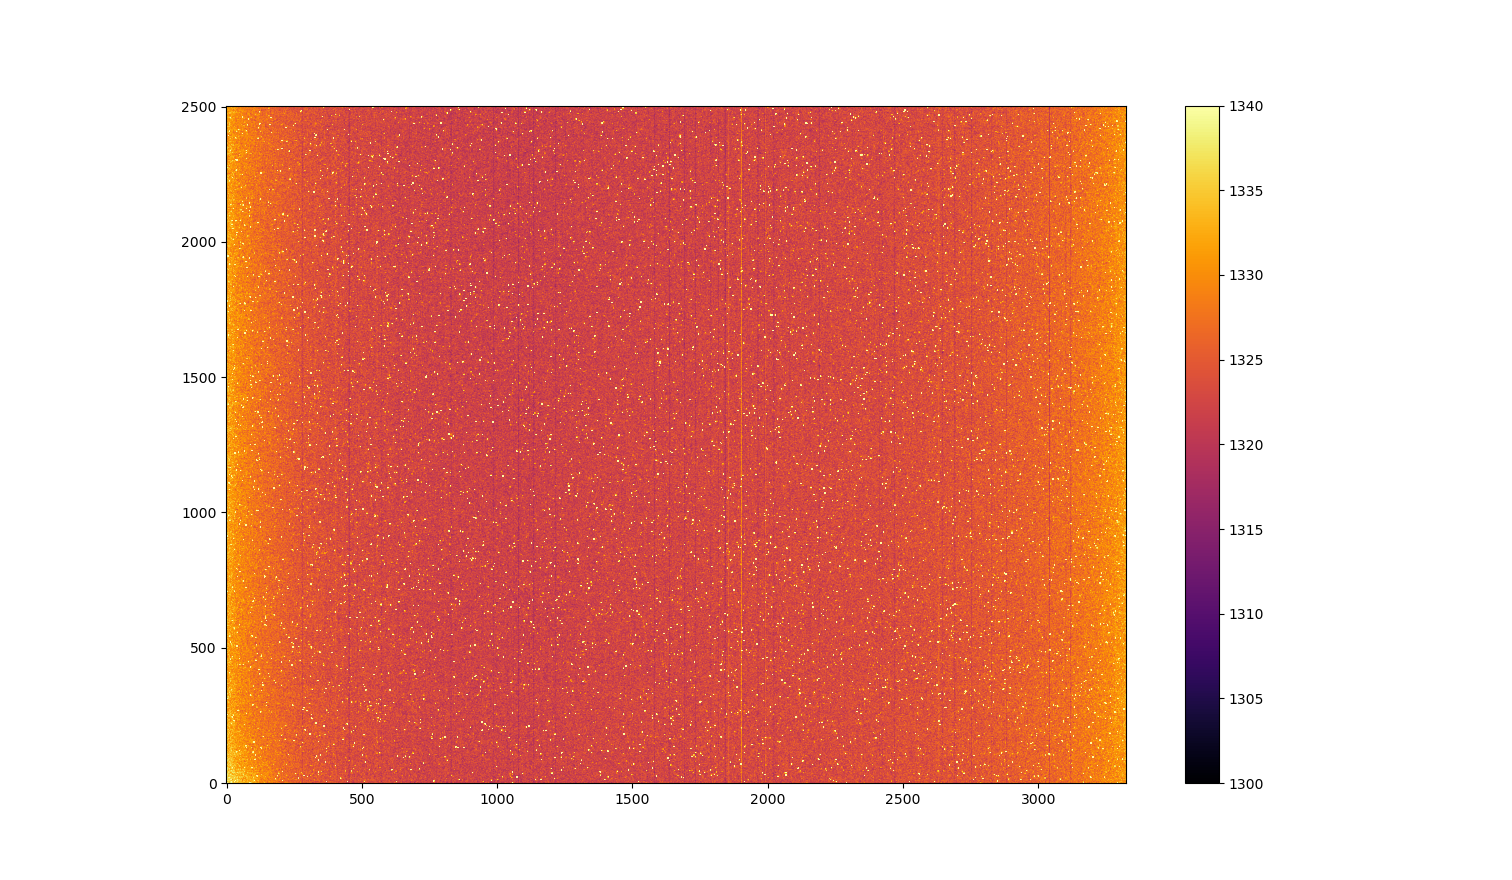
\includegraphics[width=0.9\linewidth]{bias_raw.png} 
    \caption{Bias image showing electronic noise patterns across the CCD, displayed with a range set to mean ± standard deviation.} 
    \label{fig:one_bias} 
\end{figure}

\subsection{Flat Field Images Collection}

Flat field images were collected to correct for variations in pixel sensitivity across the CCD, ensuring uniform response throughout the detector. These images were obtained by exposing the CCD to a uniformly illuminated field, enabling calibration for pixel-to-pixel sensitivity differences that could otherwise impact photometric accuracy. Flat fields were acquired in three photometric bands:
\begin{itemize}
    \item g-band: Sensitive to green wavelengths.
    \item r-band: Sensitive to red wavelengths.
    \item i-band: Sensitive to near-infrared wavelengths.
\end{itemize}
For each band, five flat field images were taken, ensuring consistent response data across the CCD. These images were combined to create a master flat field for each band. Figures~\ref{fig:g_flat_raw}, \ref{fig:r_flat_raw}, and \ref{fig:i_flat_raw} show examples of individual flat field images in the g, r, and i bands, respectively, displayed with a range based on mean and standard deviation values. These master flat fields are critical for removing systematic sensitivity variations from the science images.

\begin{figure}[h] 
    \centering 
    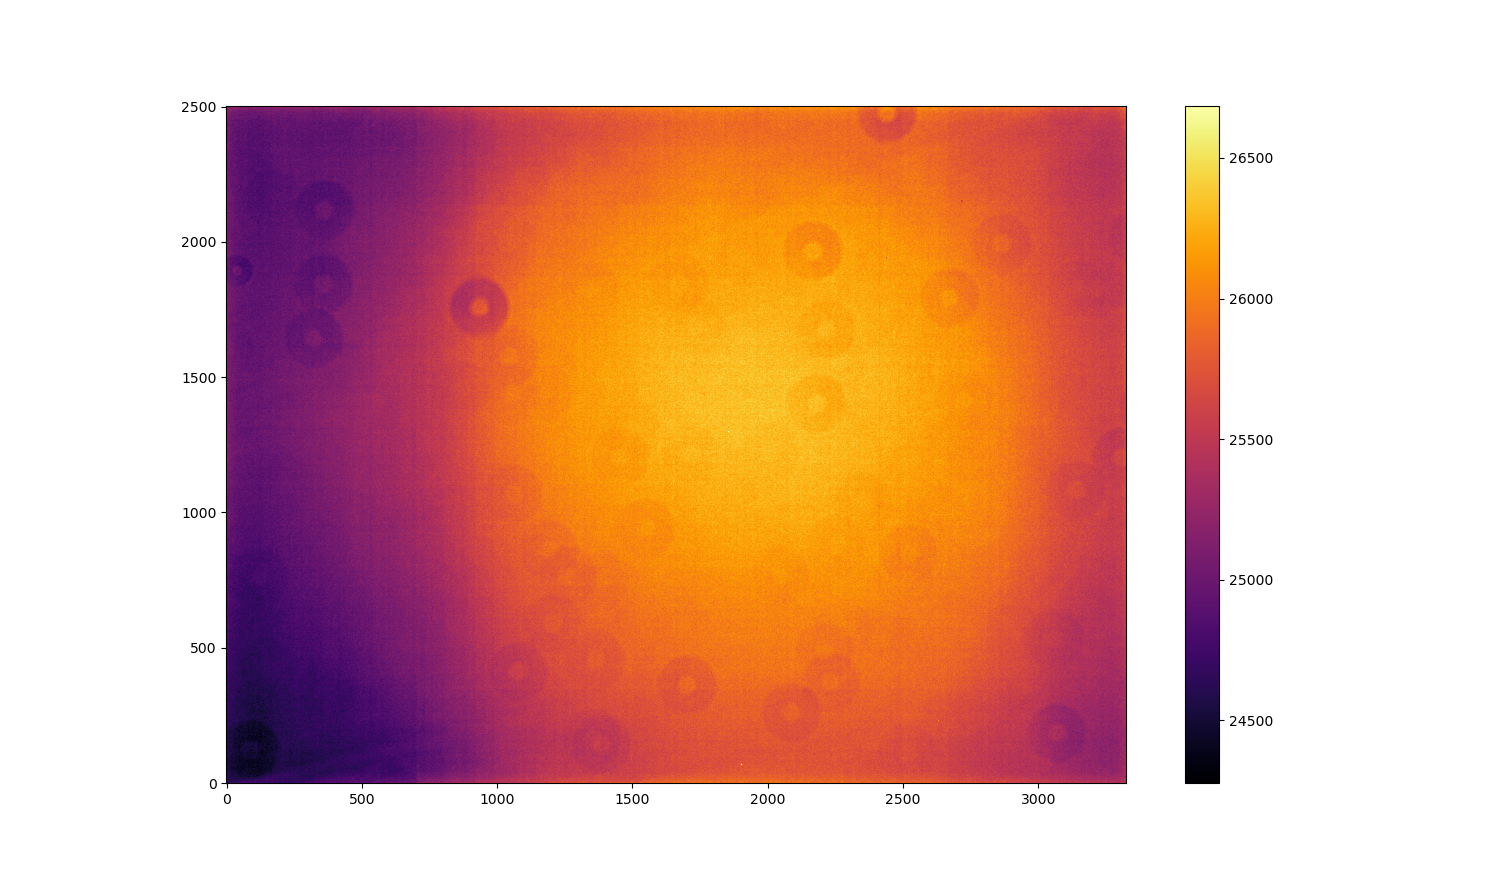
\includegraphics[width=0.9\linewidth]{g_flat_raw.png} 
    \caption{Flat field image in the g-band, showing pixel sensitivity variations across the CCD.} 
    \label{fig:g_flat_raw} 
\end{figure}

\begin{figure}[h] 
    \centering 
    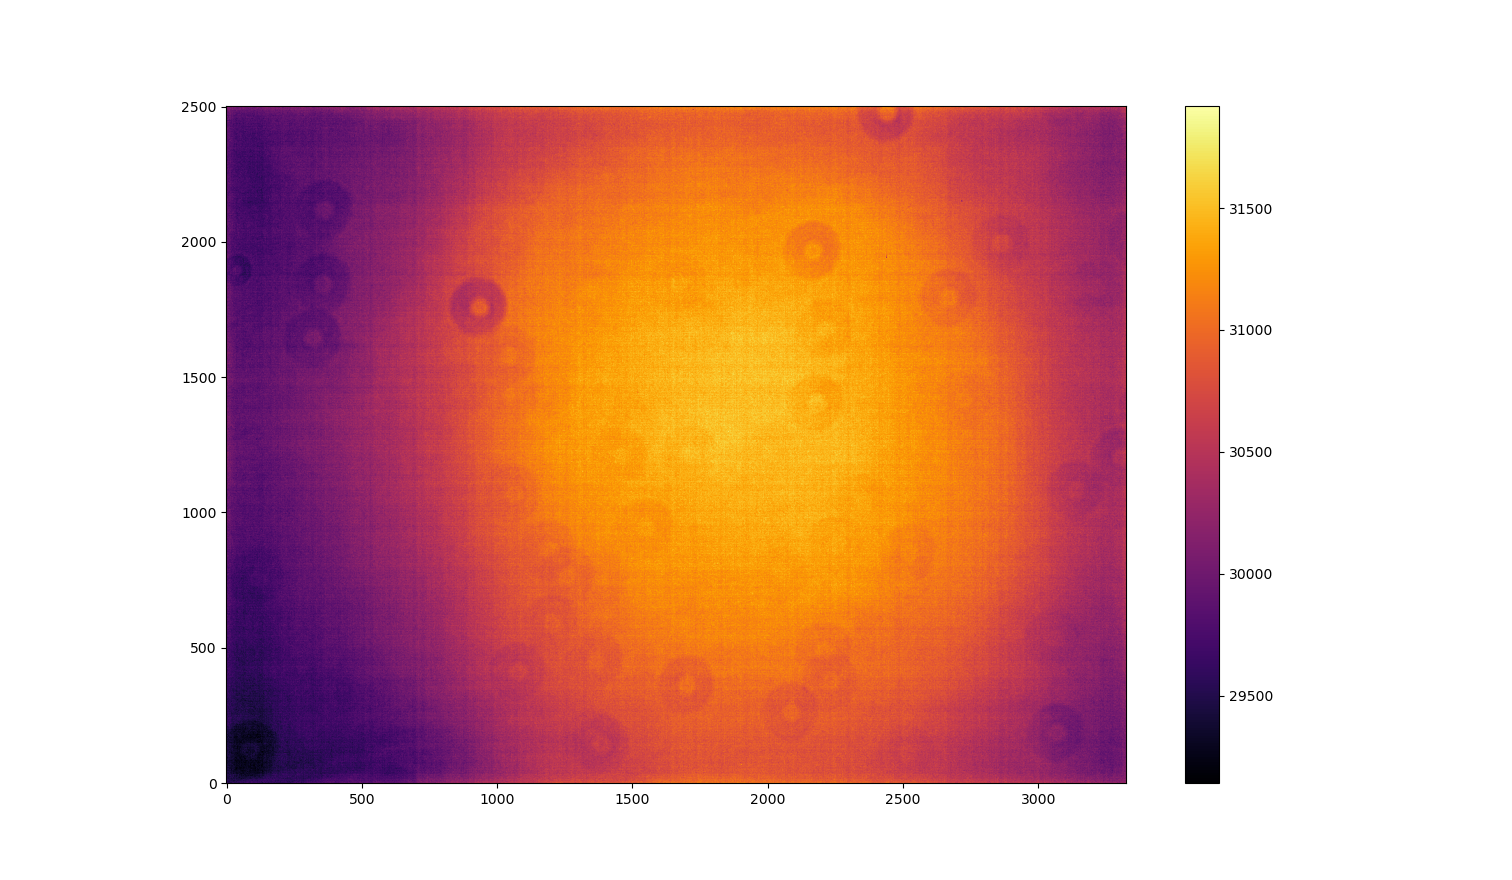
\includegraphics[width=0.9\linewidth]{r_flat_raw.png} 
    \caption{Flat field image in the r-band, showing pixel sensitivity variations across the CCD.} 
    \label{fig:r_flat_raw} 
\end{figure}

\begin{figure}[h] 
    \centering 
    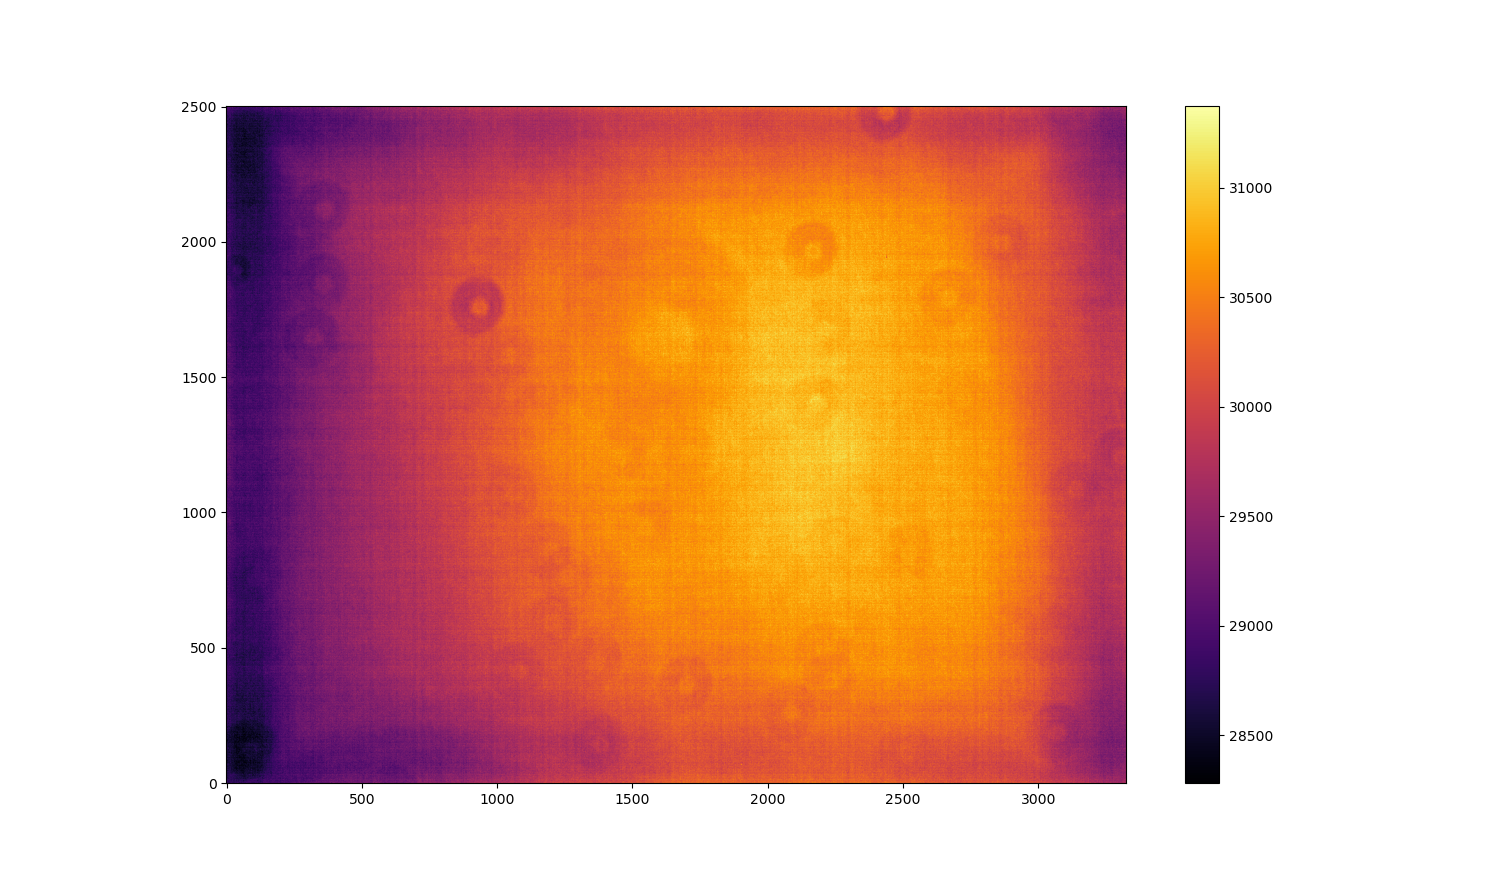
\includegraphics[width=0.9\linewidth]{i_flat_raw.png} 
    \caption{Flat field image in the i-band, showing pixel sensitivity variations across the CCD.} 
    \label{fig:i_flat_raw}
\end{figure}

\subsection{Science Images of NGC 1528}

Following the calibration data collection, we obtained science images of the star cluster NGC 1528 in the g, r, and i bands to facilitate color-magnitude analysis. We captured 5-6 science frames in each band, providing redundancy for noise reduction and ensuring sufficient data for robust photometric analysis. \\

These science images represent the core data for this lab’s photometric analysis. Once calibrated using the master bias and master flat field images, these frames will be used to extract photometric measurements and create a color-magnitude diagram for the star cluster. Figure~\ref{fig:science_raw} shows an example of a science image in one of the bands, highlighting the star cluster's field. This image provides a clear view of the target stars, which will be analyzed for photometric properties after calibration.

\begin{figure}[h] 
    \centering 
    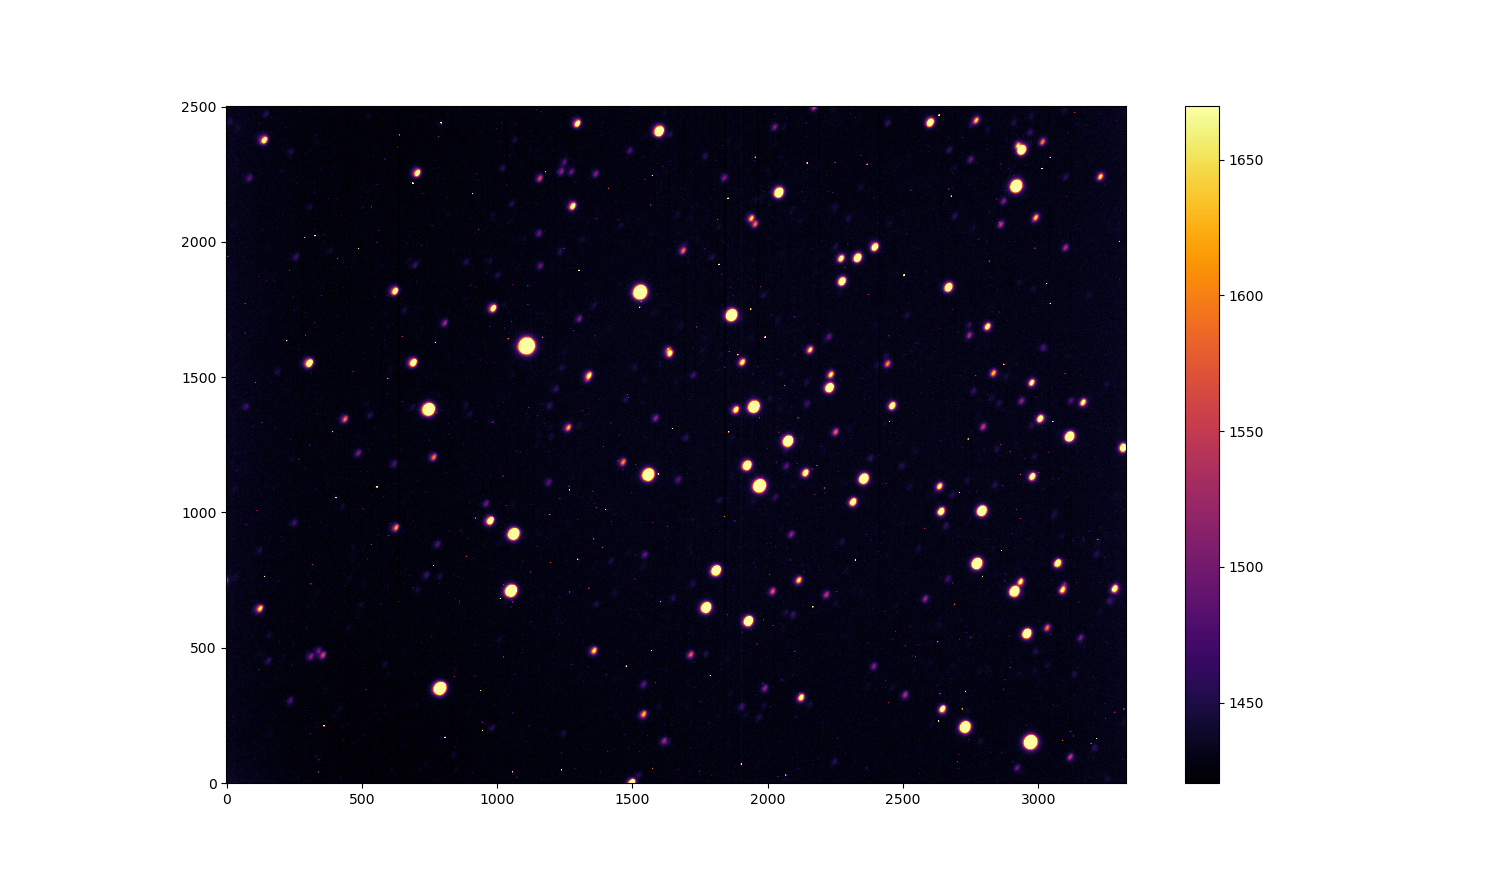
\includegraphics[width=0.9\linewidth]{science_raw.png} 
    \caption{Science image of the star cluster NGC 1528, showing the field of stars observed in the g band.} 
    \label{fig:science_raw} 
\end{figure}

\subsection{Challenges Encountered}

During initial observations, the telescope experienced tracking issues due to an incorrect parking position. We originally attempted to observe the star cluster NGC 188. However, because the telescope was not correctly parked, it was unable to accurately track the position of NGC 188, resulting in unusable data. This issue necessitated the use of data from a previous observation of the star cluster NGC 1528 for our analysis. \\

Parking the telescope correctly is crucial, as it ensures that the telescope’s alignment system can accurately locate and track celestial objects. An incorrectly parked telescope can lead to inaccurate pointing and tracking errors, making it difficult to gather reliable data. Correct parking enables the telescope to begin from a known reference position, which is essential for precise astronomical observations and minimizes the time lost on troubleshooting alignment issues.

\section{Data analysis} 
\label{sec:results}

The data analysis for this lab involved preparing calibration products, specifically the master bias and master flat field images, and applying them to the science images of the star cluster NGC 1528. The following sections describe each step up to the reduction of the science images, including the Python code used for processing.

\subsection{Creating the Master Bias Image}

The master bias image was created by stacking multiple bias frames to obtain an average representation of the baseline electronic noise in the CCD. The function \texttt{make\_master\_bias} reads all the bias frames from a specified directory and stacks them into an array. The bias frames were then averaged (or optionally the median could be used) along the stack axis to produce a single master bias image, saved as \texttt{master\_bias\_mean.fits} or \texttt{master\_bias\_median.fits} depending on the chosen method. The Python code for generating the master bias is shown below:
\begin{lstlisting}[language=Python]
import glob
import numpy as np
import astropy.io.fits as fits

class Reduce:

    def make_master_bias(bias_directory_path, mean=False):
        bias_files_list = glob.glob(bias_directory_path)
        bias_images_stack = []

        for filename in bias_files_list:
            image = fits.open(filename)[0].data.astype(float)
            bias_images_stack.append(image)

        bias_stack = np.array(bias_images_stack)

        if mean:
            master_bias = np.mean(bias_stack, axis=0)
            fits.PrimaryHDU(data=master_bias).writeto("master_bias_mean.fits", overwrite=True)
            return master_bias
        else:
            master_bias = np.median(bias_stack, axis=0)
            fits.PrimaryHDU(data=master_bias).writeto("master_bias_median.fits", overwrite=True)
            return master_bias
\end{lstlisting}

Figure~\ref{fig:master_bias} shows the master bias image created by averaging multiple bias frames. This image was subtracted from each science image to correct for electronic noise.

\begin{figure}[h]
    \centering
    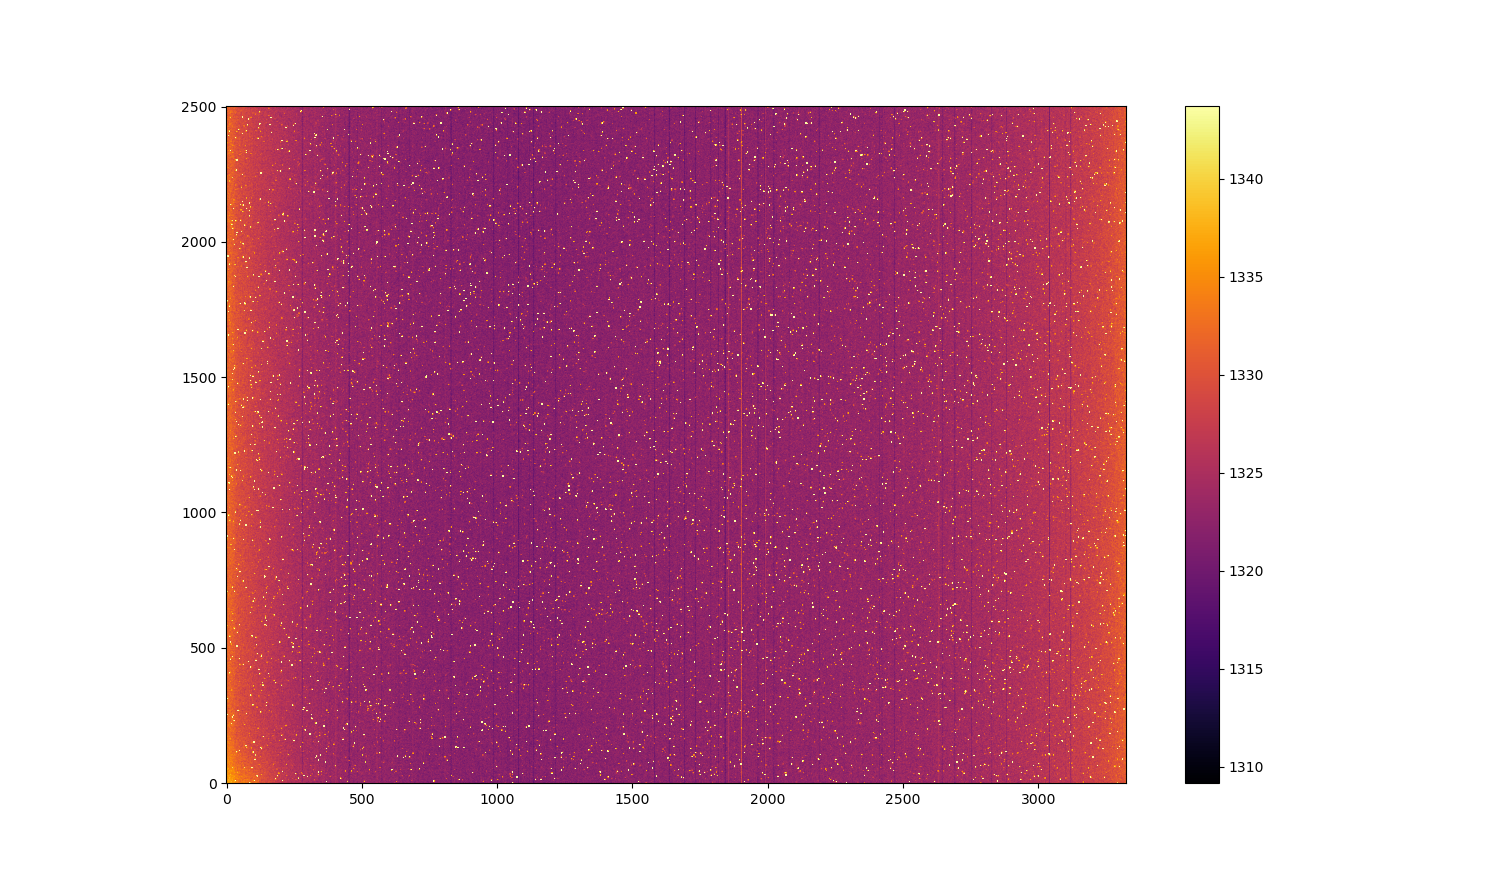
\includegraphics[width=0.9\linewidth]{master_bias.png}
    \caption{Master bias image created by averaging multiple bias frames, showing the baseline electronic noise across the CCD.}
    \label{fig:master_bias}
\end{figure}

\subsection{Creating the Master Flat Field Images}

To correct for pixel-to-pixel sensitivity variations, master flat field images were generated for each photometric band (g, r, and i). The \texttt{make\_master\_flat\_field} function reads flat field images for each band, subtracts the master bias, and normalizes each flat field by dividing it by its mean level. \\

For each band, the normalized flat field images were stacked and averaged (or the median was used as an alternative) to create a master flat field image. These master flat field images, saved as \texttt{masterflat\_g.fits}, \texttt{masterflat\_r.fits}, and \texttt{masterflat\_i.fits}, were then applied to the science images to ensure uniform response across the CCD. The code for creating the master flat fields is shown below:

\begin{lstlisting}[language=Python]
def make_master_flat_field(flat_field_directory_path, master_bias, g=True, i=True):
    flats_files_list = glob.glob(flat_field_directory_path)
    flats_images_stack = []

    for filename in flats_files_list:
        image = fits.open(filename)[0].data.astype(float)
        image = image - master_bias
        mean_level = np.mean(image)
        image = image / mean_level
        flats_images_stack.append(image)

    flats_stack = np.array(flats_images_stack)
    master_flat = np.median(flats_stack, axis=0)

    if g and not i:
        fits.PrimaryHDU(data=master_flat).writeto("masterflat_g.fits", overwrite=True)
    elif not g and not i:
        fits.PrimaryHDU(data=master_flat).writeto("masterflat_r.fits", overwrite=True)
    elif not g and i:
        fits.PrimaryHDU(data=master_flat).writeto("masterflat_i.fits", overwrite=True)

    return master_flat
\end{lstlisting}

Figures~\ref{fig:master_flat_g}, \ref{fig:master_flat_r}, and \ref{fig:master_flat_i} display the master flat field images for the g, r, and i bands, respectively.

\begin{figure}[h]
    \centering
    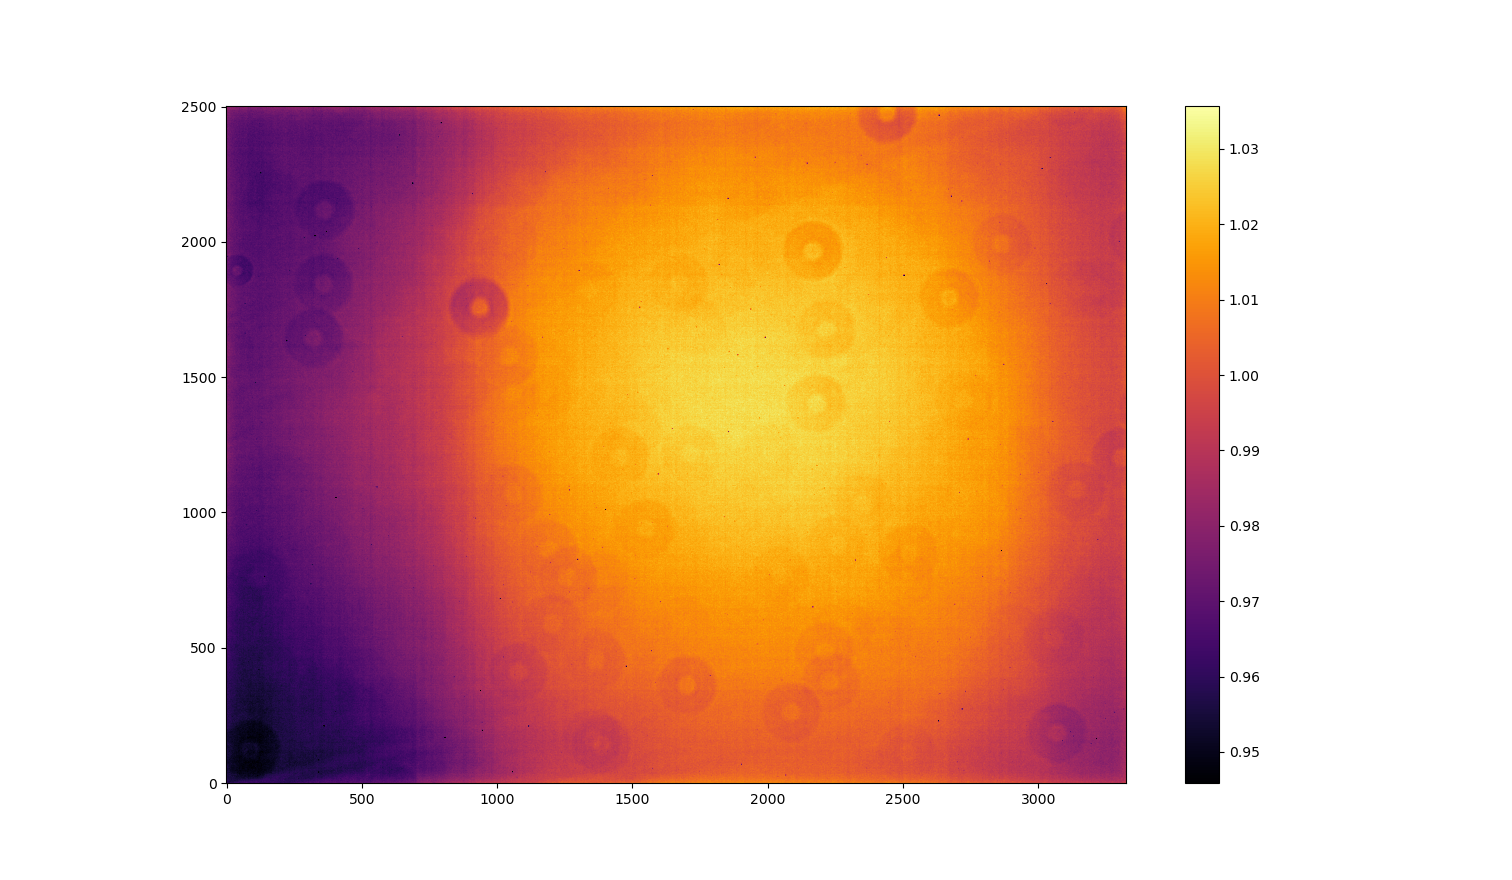
\includegraphics[width=0.9\linewidth]{master_flat_g.png}
    \caption{Master flat field image for the g-band, used to correct pixel sensitivity variations in the science images.}
    \label{fig:master_flat_g}
\end{figure}

\begin{figure}[h]
    \centering
    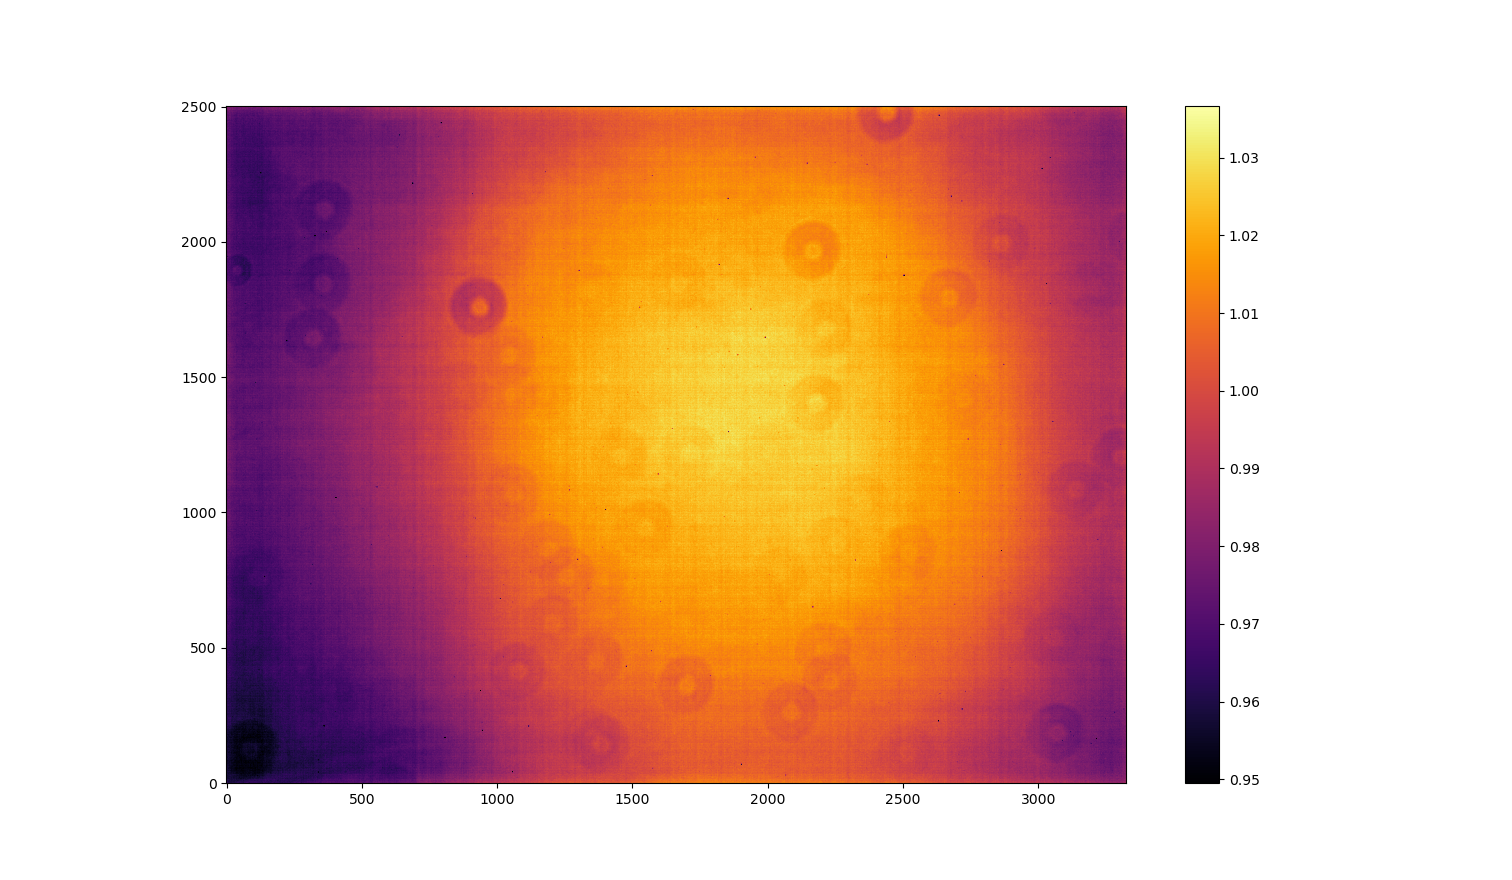
\includegraphics[width=0.9\linewidth]{master_flat_r.png}
    \caption{Master flat field image for the r-band, used to correct pixel sensitivity variations in the science images.}
    \label{fig:master_flat_r}
\end{figure}

\begin{figure}[h]
    \centering
    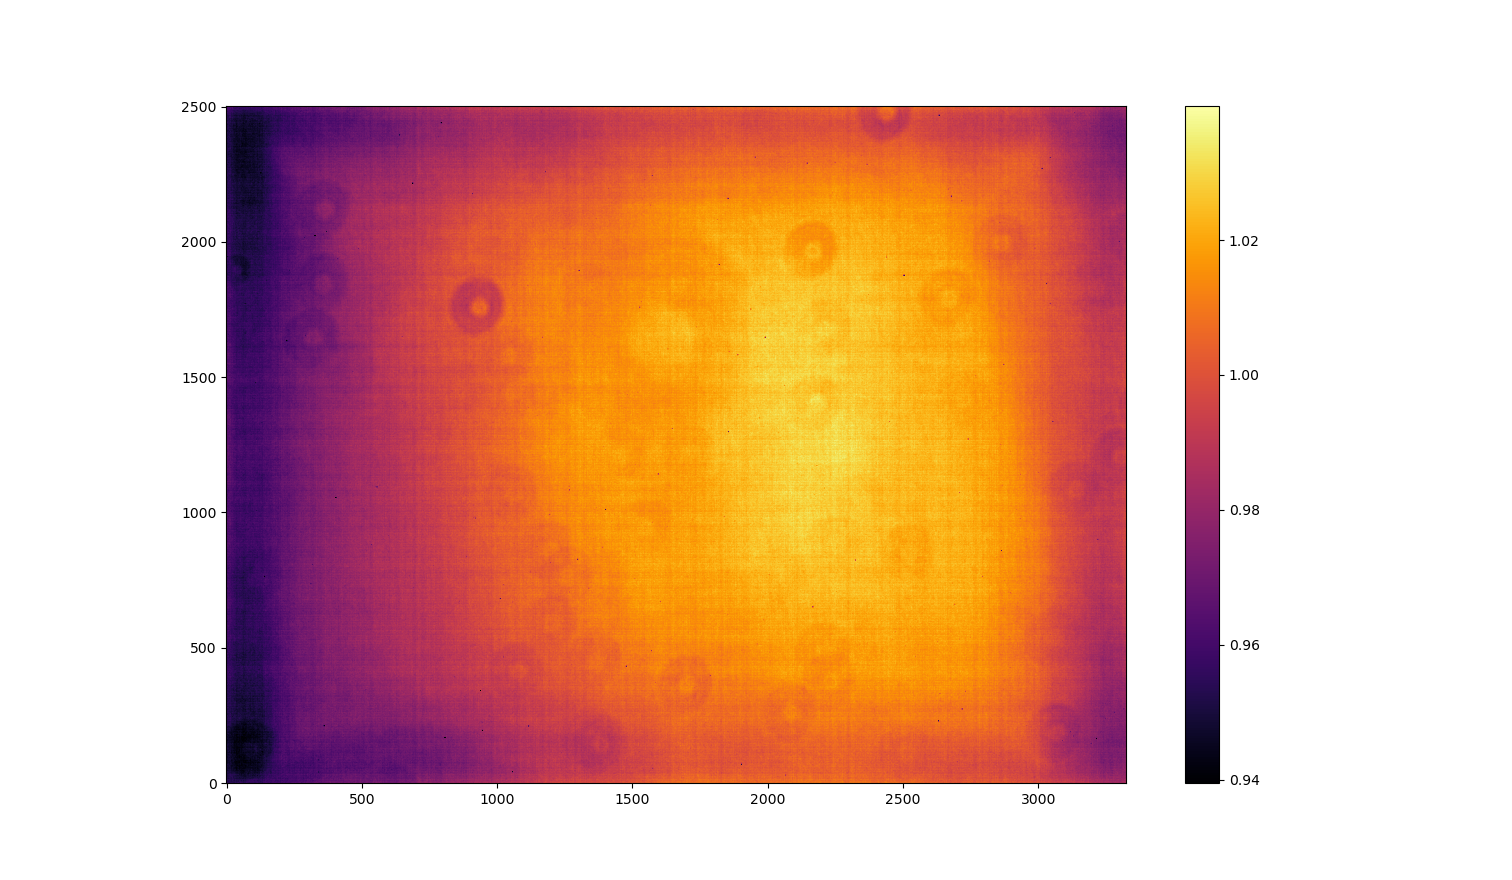
\includegraphics[width=0.9\linewidth]{master_flat_i.png}
    \caption{Master flat field image for the i-band, used to correct pixel sensitivity variations in the science images.}
    \label{fig:master_flat_i}
\end{figure}

\subsection{Reducing Science Images}

The calibrated science images were created by subtracting the master bias image and dividing by the master flat field image for each band. This process was handled by the \texttt{reduce\_science\_image} function, which takes as input a science image file, the master bias, and the corresponding master flat field. \\

The function first subtracts the master bias from the raw science image, removing electronic noise, and then divides by the master flat field to correct for pixel sensitivity variations. This process was repeated for all science images across the g, r, and i bands, yielding reduced images suitable for photometric analysis. The Python code for reducing science images is shown below:

\begin{lstlisting}[language=Python]
def reduce_science_image(science_image_path, master_bias, master_flat):
    image = fits.open(science_image_path)[0].data.astype(float)
    image = image - master_bias
    image = image / master_flat
    return image
\end{lstlisting}

Figures~\ref{fig:reduced_g}, \ref{fig:reduced_r}, and \ref{fig:reduced_i} display examples of reduced science images in the g, r, and i bands, respectively. These calibrated images are prepared for further photometric analysis.

\begin{figure}[h]
    \centering
    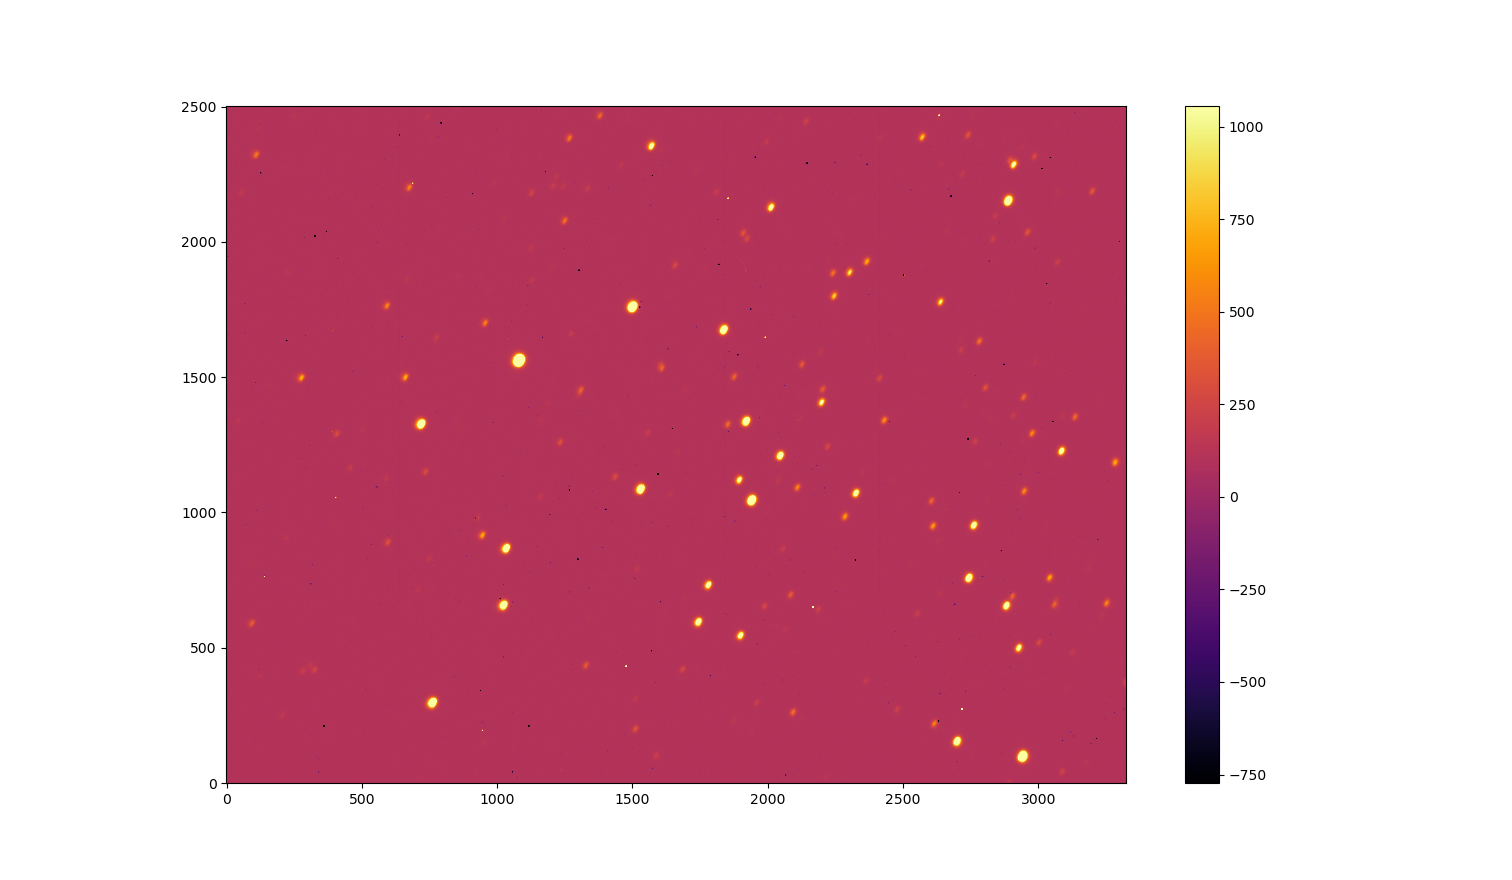
\includegraphics[width=0.9\linewidth]{reduced_science_g.png}
    \caption{Reduced science image in the g-band after bias subtraction and flat field correction.}
    \label{fig:reduced_g}
\end{figure}

\begin{figure}[h]
    \centering
    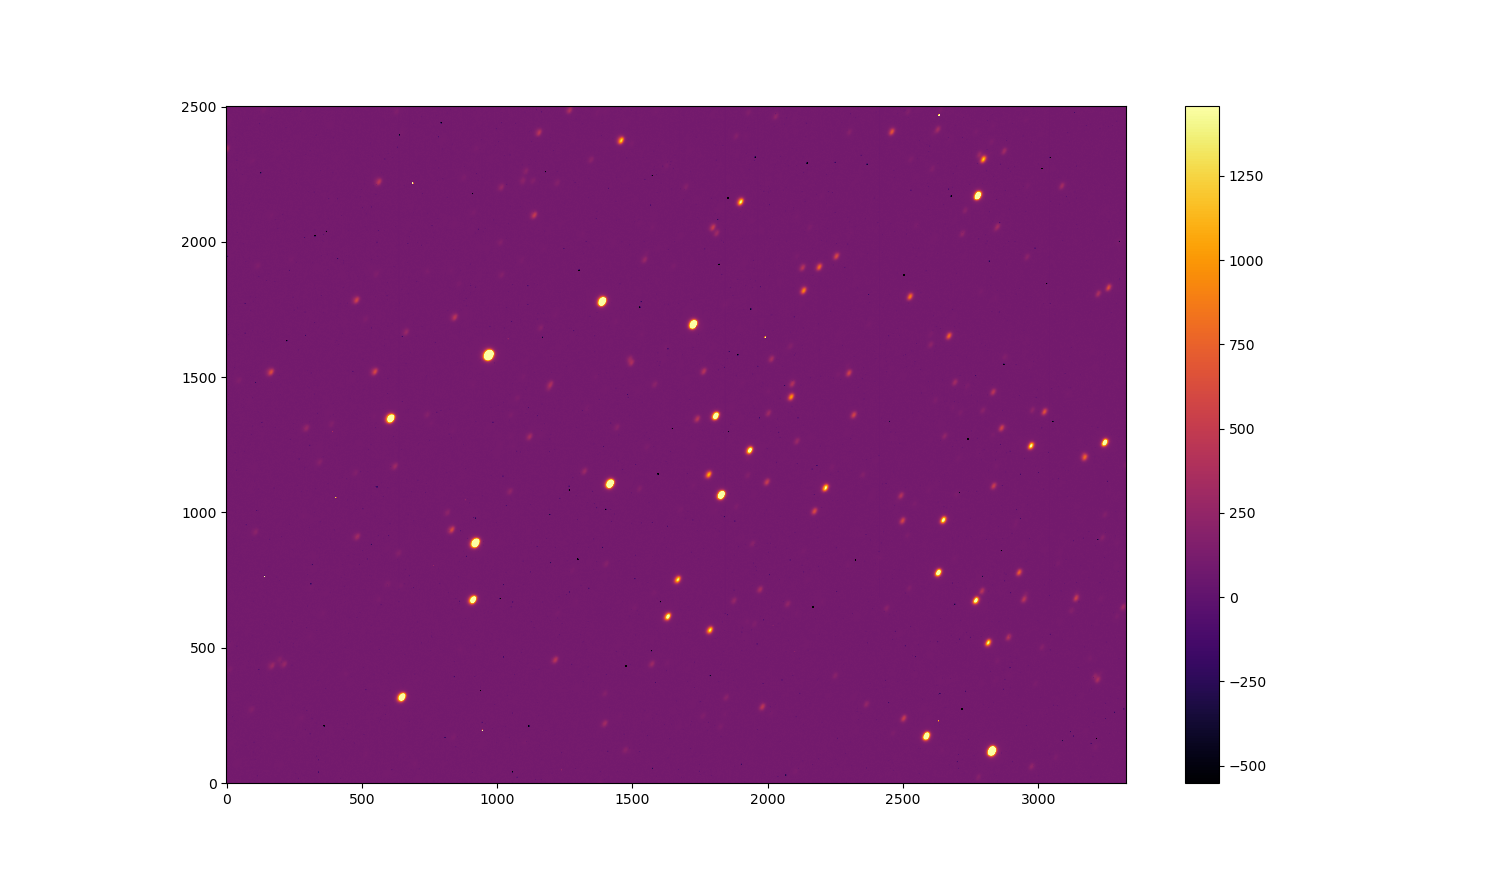
\includegraphics[width=0.9\linewidth]{reduced_science_r.png}
    \caption{Reduced science image in the r-band after bias subtraction and flat field correction.}
    \label{fig:reduced_r}
\end{figure}

\begin{figure}[h]
    \centering
    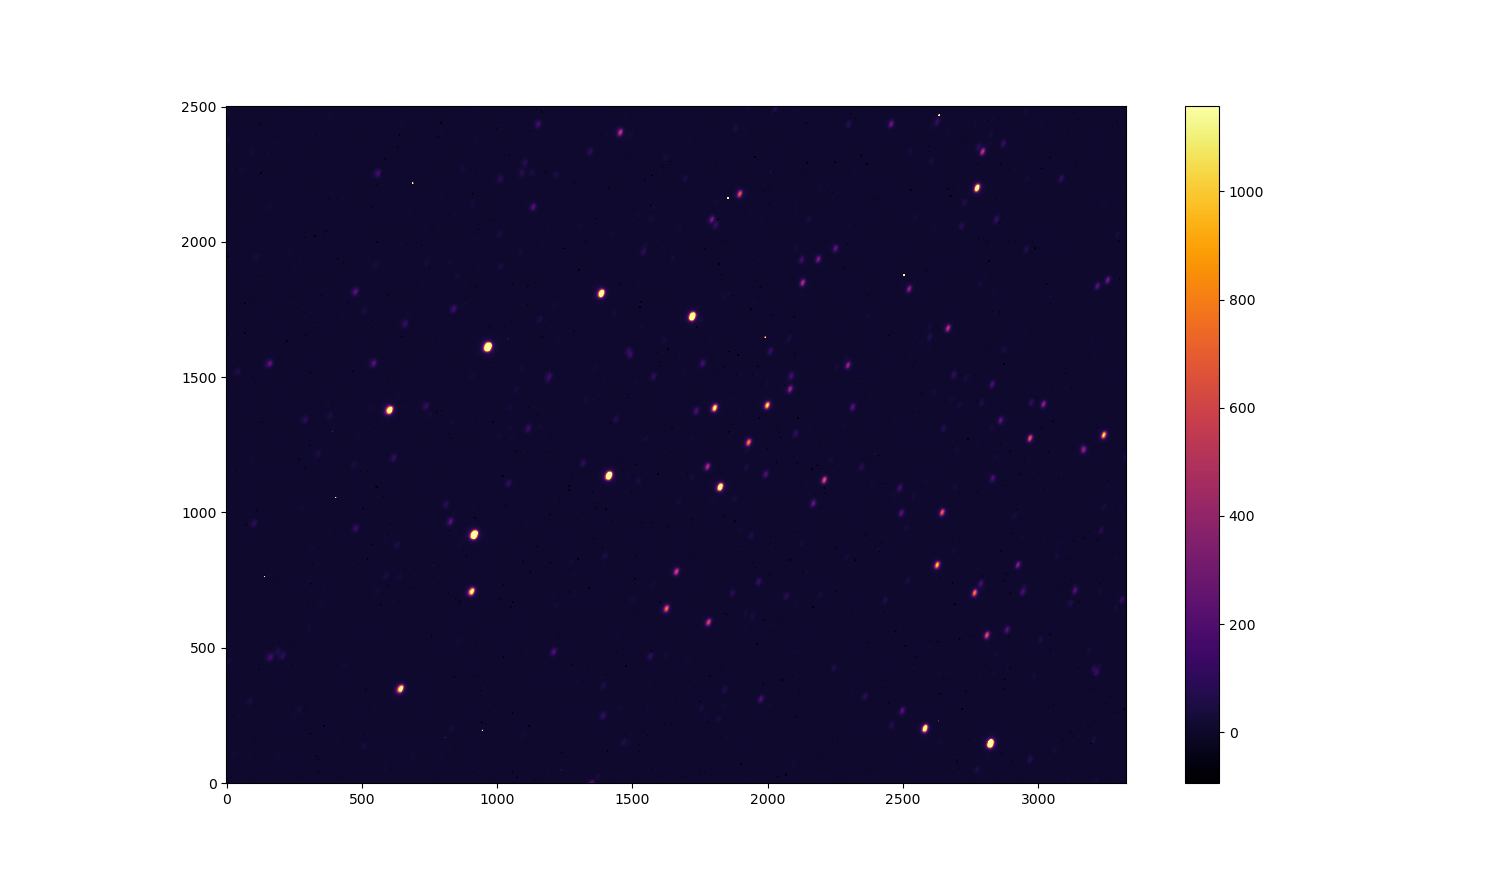
\includegraphics[width=0.9\linewidth]{reduced_science_i.png}
    \caption{Reduced science image in the i-band after bias subtraction and flat field correction.}
    \label{fig:reduced_i}
\end{figure}

\section{Conclusions}

In this lab, we undertook a comprehensive process to analyze the star cluster NGC 1528 through photometric techniques, requiring careful calibration and data reduction steps. Each phase of the lab, from observational setup to data reduction, was essential for ensuring the scientific integrity of our results. Below, we summarize the key findings and outcomes of each section.

\subsection{Observational Setup and Data Collection}

The observations of star cluster NGC 1528 were conducted using a CCD telescope controlled through a Raspberry Pi with Astroberry and CCDeil software. This setup allowed precise adjustments to exposure time, filter selection, and CCD settings, which were crucial for obtaining high-quality calibration and science images. Bias frames were captured to measure baseline electronic noise, and flat field images were taken in the g, r, and i bands to account for variations in pixel sensitivity. These calibration images laid the groundwork for reducing and refining the raw data, enabling reliable photometric analysis.

\subsection{Data Reduction and Calibration}

The data reduction process involved creating master bias and master flat images, which were critical for eliminating systematic errors. The master bias image, generated by averaging individual bias frames, allowed us to remove the baseline electronic noise inherent to the CCD detector. Meanwhile, the master flat fields, created for each band, corrected for variations in pixel response, ensuring a uniform detector sensitivity across all pixels. These steps collectively enabled us to produce clean, calibrated science images that are essential for accurate brightness measurements of stars in NGC 1528.

\subsection{Preparation for Photometric Analysis}

After applying the master bias and master flat fields, the science images were fully calibrated and ready for photometric analysis. These reduced images, now free from electronic noise and pixel sensitivity artifacts, form a reliable dataset that can be used to extract stellar brightness and color information. Such information is fundamental for constructing color-magnitude diagrams, which provide insights into the star cluster’s stellar population, including estimates of age, metallicity, and evolutionary stage.

\subsection{Overall Importance of the Data Reduction Process}

The careful data reduction process employed in this lab is foundational in astrophotography and scientific imaging. By methodically calibrating our images, we have minimized systematic errors, enabling accurate and unbiased photometric measurements. These calibrated images allow for robust analysis and facilitate scientific conclusions regarding the properties of star clusters. The techniques learned in this lab, from observational setup to calibration, emphasizes the importance of systematic data processing in astronomical studies.

\subsection{Summary}

Through a systematic approach to data collection, calibration, and reduction, this lab provided a comprehensive understanding of the steps required for accurate photometric analysis. The combination of observational planning, technical calibration, and data processing has equipped us with the skills to derive scientifically valid conclusions about stellar populations. The methods applied here, serve as a vital toolset for understanding celestial objects and their physical properties with precision. \\

This lab serves as a stepping stone for future photometric projects, providing a structured approach that can be applied to the analysis of other star clusters and celestial phenomena, thereby deepening our understanding of the universe.

\section{References}

\begin{enumerate}
    \item University of Wisconsin-Madison, \textit{Astronomy 465: Optical Astronomy Lab Manual}. University of Wisconsin-Madison, Department of Astronomy, 2024.
    
    \item University of Wisconsin-Madison, \textit{Astron 465 Lecture Slides}. University of Wisconsin-Madison, Department of Astronomy, 2024. Accessed during lectures.

    \item Howell, S. B. \textit{Handbook of CCD Astronomy}, 2nd edition. National Optical Astronomy Observatory and WIYN Observatory, 2006.

    \item University of Wisconsin-Madison, \textit{Sterling Rooftop Observatory Manual}. University of Wisconsin-Madison, Department of Astronomy, 2024.
\end{enumerate}

\end{document}